\documentclass[dvipdfmx,11pt]{beamer}		% for my notebook computer and my Mac computer
%\documentclass[11pt]{beamer}			% for overleaf

\usepackage{amsmath}
\usepackage{amssymb}
%\usepackage{amsthm}
\usepackage{multicol}
\usepackage{listings}
\usepackage{otf}
\usepackage{algorithm}
\usepackage{algorithmic}
\usepackage{tikz}
\usepackage{mathtools}
\usepackage{comment}
\usetheme{Berlin}	%全体のデザイン

\useoutertheme[subsection=false]{smoothbars}	%デザインのカスタマイズ

\setbeamertemplate{navigation symbols}{}	%右下のちっちゃいナビゲーション記号を非表示

\AtBeginSection[]	%サブセクションごとに目次を表示
{\begin{frame}{Contents}
    \begin{multicols}{2}
        \tableofcontents[currentsubsection]
    \end{multicols}
\end{frame}}
\newtheorem{defi}{Definition}
\newtheorem{thm}[defi]{Theorem}
\newtheorem{prop}[defi]{Proposition}
\newtheorem{conj}[defi]{Conjecture}
\newtheorem{exam}[defi]{Example}
\newtheorem{prob}[defi]{Problem}
\newtheorem{set}[defi]{Setting}
\newtheorem{claim}[defi]{Claim}

\newcommand{\N}{\mathbb{N}}
\newcommand{\R}{\mathbb{R}}
\newcommand{\X}{\mathcal{X}}
\newcommand{\Y}{\mathcal{Y}}

\newcommand{\tpm}{T_xM}


\newcommand{\argmax}{\mathop{\rm arg~max}\limits}
\newcommand{\argmin}{\mathop{\rm arg~min}\limits}



%---------------数理最適化--------------
\newcounter{mpproblem}[section]
\renewcommand{\thempproblem}{\thesection.\arabic{mpproblem}}
\makeatletter
\newenvironment{mpproblem}[1]%
{%
    \protected@edef\@currentlabelname{#1}%
    \par\vspace{\baselineskip}\noindent%
    \ifx#1\empty %
    \else \refstepcounter{mpproblem}$($#1$)$ %
    \fi%
    \hfill%
    $\left|%
    \hfill%
    \hspace{0.00\textwidth}%
    \@fleqntrue\@mathmargin\parindent%
    \begin{minipage}{0.86\textwidth}%
    \vspace{-1.0\baselineskip}%
}%
{%
    \end{minipage}%
    \@fleqnfalse%
    \right.$%
    \par\vspace{\baselineskip}\noindent%
    \ignorespacesafterend%
}%
\makeatother
\newcommand{\mpprobref}[1]{$($\nameref{#1}$)$}
\newenvironment{mpproblem*}%
{%
    \begin{mpproblem}{}%
}%
{%
    \end{mpproblem}%
    \ignorespacesafterend%
}
%-----------------------------------

\title{Optimization Algorithm on Riemannian Manifolds}
\author{小泉孝弥}
\institute{立命館大学大学院 修士2年}
\date{\today}
\begin{document}
    \begin{frame}\frametitle{}
        \titlepage
    \end{frame}

    \section{Introduction}
    \begin{frame}
        \frametitle{Introduction}
        本発表では制約空間$M$がリーマン多様体となっている非線形連続最小化問題を扱う. すなわち, 
        関数$f : \R^n\to\R$が与えられたとき, 
        \begin{mpproblem*}
            \begin{alignat*}{2}
                &\text{minimize}   & f(x)  \\
                &\text{subject to } & x\in M  
            \end{alignat*}
        \end{mpproblem*}
        制約空間$M$がリーマン多様体となっている場合, $f$を$M$に制限することで, 制約なしの問題と考えることができる. 
        今回は, 勾配降下法をリーマン多様体上に拡張し, 数値計算を行なった結果を報告する.
    \end{frame}

    \section{Riemmannian Manifold and Examples}
    \subsection{Definiton and Gradient}
    \begin{frame}\frametitle{Riemmannian Manifold}
        \begin{defi}[Riemmannian Manifold]
            $M$を可微分多様体とする. 各点$x\in M$の接空間$\tpm$に内積$g_x : \tpm\times\tpm\to\R$が定まっているとき, 
            $g = (f_x)_{x\in M}$をリーマン計量と呼び, 組$(M, g)$をリーマン多様体(Riemmannian Manifold)という.
        \end{defi}
        \begin{defi}[Gradient]
            $(M, g)$をリーマン多様体とし, $f:M\to\R$を可微分関数とする. $x\in M$について
            $f$の$x$での勾配$\mathrm{grad}f(x)\in\tpm$を以下で定める.
            \begin{align*}
                \forall\xi\in\tpm, g(\mathrm{grad}f(x), \xi) = Df(x)[\xi]
            \end{align*}
        \end{defi}
    \end{frame}
    \subsection{Examples}
    \begin{frame}\frametitle{Sphere}
        \begin{exam}[Sphere]
            自然数$n\geq2$に対して, 球面$S^{n - 1}\coloneqq\{x\in\R^n\mid x^{\top}z = 0\}$
            は可微分多様体となる. また, $x\in S^{n - 1}$での接空間$T_xS^{n-1}$は
            \begin{align*}
                T_xS^{n - 1} = \{z\in\R^n\mid x^{\top}z = 0\}
            \end{align*}
            となる. ここで, $g_x : T_xS^{n - 1}\times T_xS^{n - 1}\to\R$を
            \begin{align*}
                g_x(\xi, \eta) = \xi^{\top}\eta
            \end{align*}
            と定めれば, $g_x$は$T_xS^{n-1}$の内積となるので, $S^{n - 1}$はリーマン多様体である.
        \end{exam}
    \end{frame}
    \begin{frame}\frametitle{Stiefel Manifold}
        \begin{exam}[Stiefel Manifold]
            $X = [x_1x_2\ldots x_p]\in\R^{n\times p}(n\geq p)$で, $\{x_i\}_{i = 1}^p\subset\R^n$が正規直交系であるような
            $n\times p$行列全体は可微分多様体となる. この多様体をシュティーフェル多様体(Stiefel Manifold)といい, 
            $\operatorname{St}(p, n)$と表す. すなわち
            \begin{align*}
                \operatorname{St}(p, n) = \{X\in\R^{n\times p}\mid X^{\top}X = \mathbb{I}_{p}\}.
            \end{align*}
            である.
        \end{exam}
    \end{frame}

    \begin{frame}\frametitle{}
        $X\in\operatorname{St}(p, n)$での接空間$T_{X}St(p, n)$は, 
        \begin{align*}
            T_{X} \operatorname{St}(p, n)&=\left\{Z \in \mathbb{R}^{n \times p}\mid X^{T} Z+Z^{T} X=0\right\}\\
                                         &= \left\{X \Omega+X_{\perp} K\mid \Omega\in\operatorname{Skew}(p), K \in \mathbb{R}^{(n-p) \times p}\right\}
        \end{align*}
        となる. ここで$\operatorname{Skew}(p) = \{\Omega\in\R^{p\times p}\mid \Omega^{\top} = -\Omega\}$であり, 
        $X_{\perp}$は$\operatorname{span}(X)^{\perp} = \operatorname{span}(X_{\perp})$を満たす$n\times (n - p)$行列である.
        $g_{X} : T_{X}\operatorname{St}(p, n)\times T_{X}\operatorname{St}(p, n)\to\R$を,
        \begin{align*}
            g_{X}(\xi, \eta) = \operatorname{tr}(\xi^{\top} \eta)
        \end{align*}
        と定めれば, $g_{X}$は内積となるので, $\operatorname{St}(p, n)$はリーマン多様体である. 
    \end{frame}

    
   
    \section{Extension to Riemannian Manifold}

    \begin{frame}

        \frametitle{Gradient Decent}
        \begin{algorithm}[H]
            \caption{Gradient Decent(GD)}
            \begin{algorithmic}
                \REQUIRE $f$: differentiable function on $\R^{n}$
                \REQUIRE $0< t <1$ : 
                \STATE $x\leftarrow x_{0}\in\R^n$
                \WHILE{$x$ not converged} 
                \STATE $x\leftarrow x - t~\mathrm{grad}_{\R^n} f(x)\in\R^n$ 
                \ENDWHILE
                \RETURN $x$
            \end{algorithmic}
        \end{algorithm}
    \end{frame}
    \begin{frame}\frametitle{Motivation}
        勾配降下法を制約空間がユークリッド空間に埋め込まれたリーマン部分多様体に拡張する. その際に, 勾配の部分をリーマン多様体上の勾配に変更
        するだけでは, リーマン多様体からはみ出てしまうため, 制約条件を満たすことが出来ない. そこで, はみ出てしまった点を
        リーマン多様体に戻す写像を考えることで, 制約を満たす点列$\{x_k\}$を得ることができる.
        \begin{figure}
            \centering
            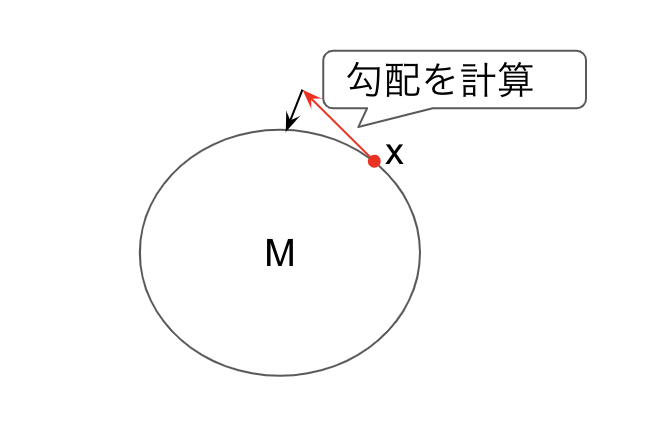
\includegraphics[width = 5.5cm]{../Images/retraction_flow.png}
        \end{figure}
    \end{frame}

    \begin{frame}

        \frametitle{Gradient Decent}
        \begin{algorithm}[H]
            \caption{Gradient Decent(GD)}
            \begin{algorithmic}
                \REQUIRE $f$: differentiable function on $\R^{n}$
                \REQUIRE $0< t <1$ : 
                \STATE $x\leftarrow x_{0}\in M$
                \WHILE{$x$ not converged} 
                \STATE $x\leftarrow x - t~\mathrm{grad} f(x){\color{red}\notin M}$ 
                \ENDWHILE
                \RETURN $x$
            \end{algorithmic}
        \end{algorithm}
    \end{frame}

    \subsection{Retraction}
    \begin{frame}\frametitle{Retraction}
        リーマン多様体$M$に対して, 接束を$\displaystyle TM = \bigcup_{x\in M}\tpm$と表す.
        \begin{defi}[Retraction]
            $M$をリーマン多様体, $R : TM\to M$を$C^\infty$写像とする. 
            任意の$x\in M$に対して, $R$の$\tpm$への制限$R_x : \tpm\to M$が以下の2つの条件を満たすとき, $R$
            を$M$上のレトラクション(Retraction)と呼ぶ.
            \begin{enumerate}
                \item $R_x(0_x) = x$
                \item $DR_x(0_x) = id_{\tpm}$
            \end{enumerate}
        \end{defi}
    \end{frame}


    \subsection{Riemannian Gradient Decent Method}
    
    \begin{frame}\frametitle{Riemannian Gradient Decent}
        $M$をリーマン多様体, $R : TM\to M$をレトラクションとする.
        リーマン多様体上の勾配降下法(RGD)を以下のように設計する.
        \begin{algorithm}[H]
            \caption{Riemannian Gradient Decent(RGD)}
            \begin{algorithmic}
                \REQUIRE $f$: differentiable function on $M$
                \REQUIRE $0< t <1$ : 
                \STATE $x\leftarrow x_{0}\in M$
                \WHILE{$x$ not converged} 
                \STATE $x\leftarrow R_x(-t~\mathrm{grad} f(x))$ 
                \ENDWHILE
                \RETURN $x$
            \end{algorithmic}
        \end{algorithm}
    \end{frame}
    \section{Numerical Experiments}
    
    \subsection{Minimation of quadratic form}
    \begin{frame}
        \frametitle{二次形式の最小化}
        \begin{block}{二次形式の最小化問題}
            $A\in\R^{n\times n}$を対称行列とする. 
            \begin{mpproblem*}
                \begin{alignat*}{2}
                    &\text{minimize}   & q_A(x) = x^{\top}Ax  \\
                    &\text{subject to } & x\in S^{n - 1}  
                \end{alignat*}
            \end{mpproblem*}
        \end{block}
        なお, $\displaystyle \min_{x\in S^{n - 1}} q_A(x)$は$A$の最小固有値, $\argmin_{x\in S^{n - 1}}q_A(x)$は最小固有値に対する固有ベクトル
        となる.
    \end{frame}

    \begin{frame}
        \frametitle{Result}
        レトラクション$R$以下で定義する. 
        \begin{align*}
            R_x(\xi) = \frac{x + \xi}{\|x + \xi\|}
        \end{align*} 
        \begin{figure}[b]
            \begin{tabular}{c}
                \begin{minipage}{0.55\hsize}
                    \centering
                    \caption{n = 100}
                    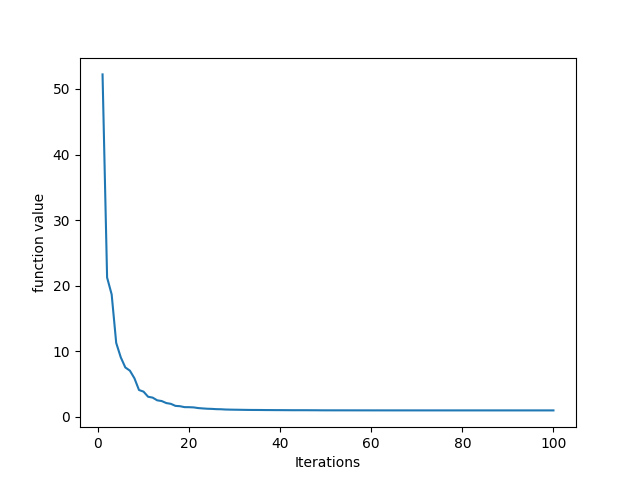
\includegraphics[width = 5.0cm]{../Images/quad_100.png}
                \end{minipage}
                \begin{minipage}{0.45\hsize}
                    \centering
                    \caption{n = 2000}
                    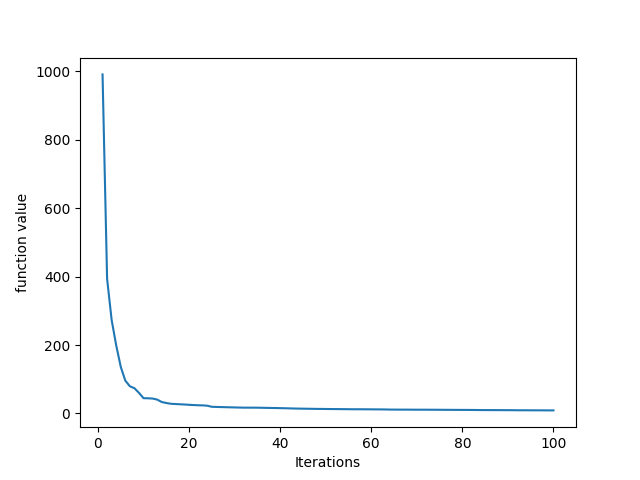
\includegraphics[width = 5.0cm]{../Images/quad_2000.png}
                \end{minipage}
            \end{tabular}   
        \end{figure}  
    \end{frame}

    \section*{References}
    \begin{frame}\frametitle{References}
        \begin{thebibliography}{9}
            \beamertemplatetextbibitems
            \bibitem{absil} P.-A. ABSIL, R. MAHONY, AND R. SEPULCHRE, Optimization Algorithms on Matrix Manifolds, 
                       Princeton University Press, Princeton, NJ, 2008.
	    \end{thebibliography}
    \end{frame}
\end{document}